\FloatBarrier

\section*{Appendix}

\subsection*{High-feature diagnostic trajectories}
The main Results section uses low-feature diagnostic panels to keep the visual narrative focused on the regimes
where successive neurons are easiest to inspect. For completeness, the corresponding high-feature panels are
shown below for both benchmarks.

\begin{figure}[!htbp]
\centering
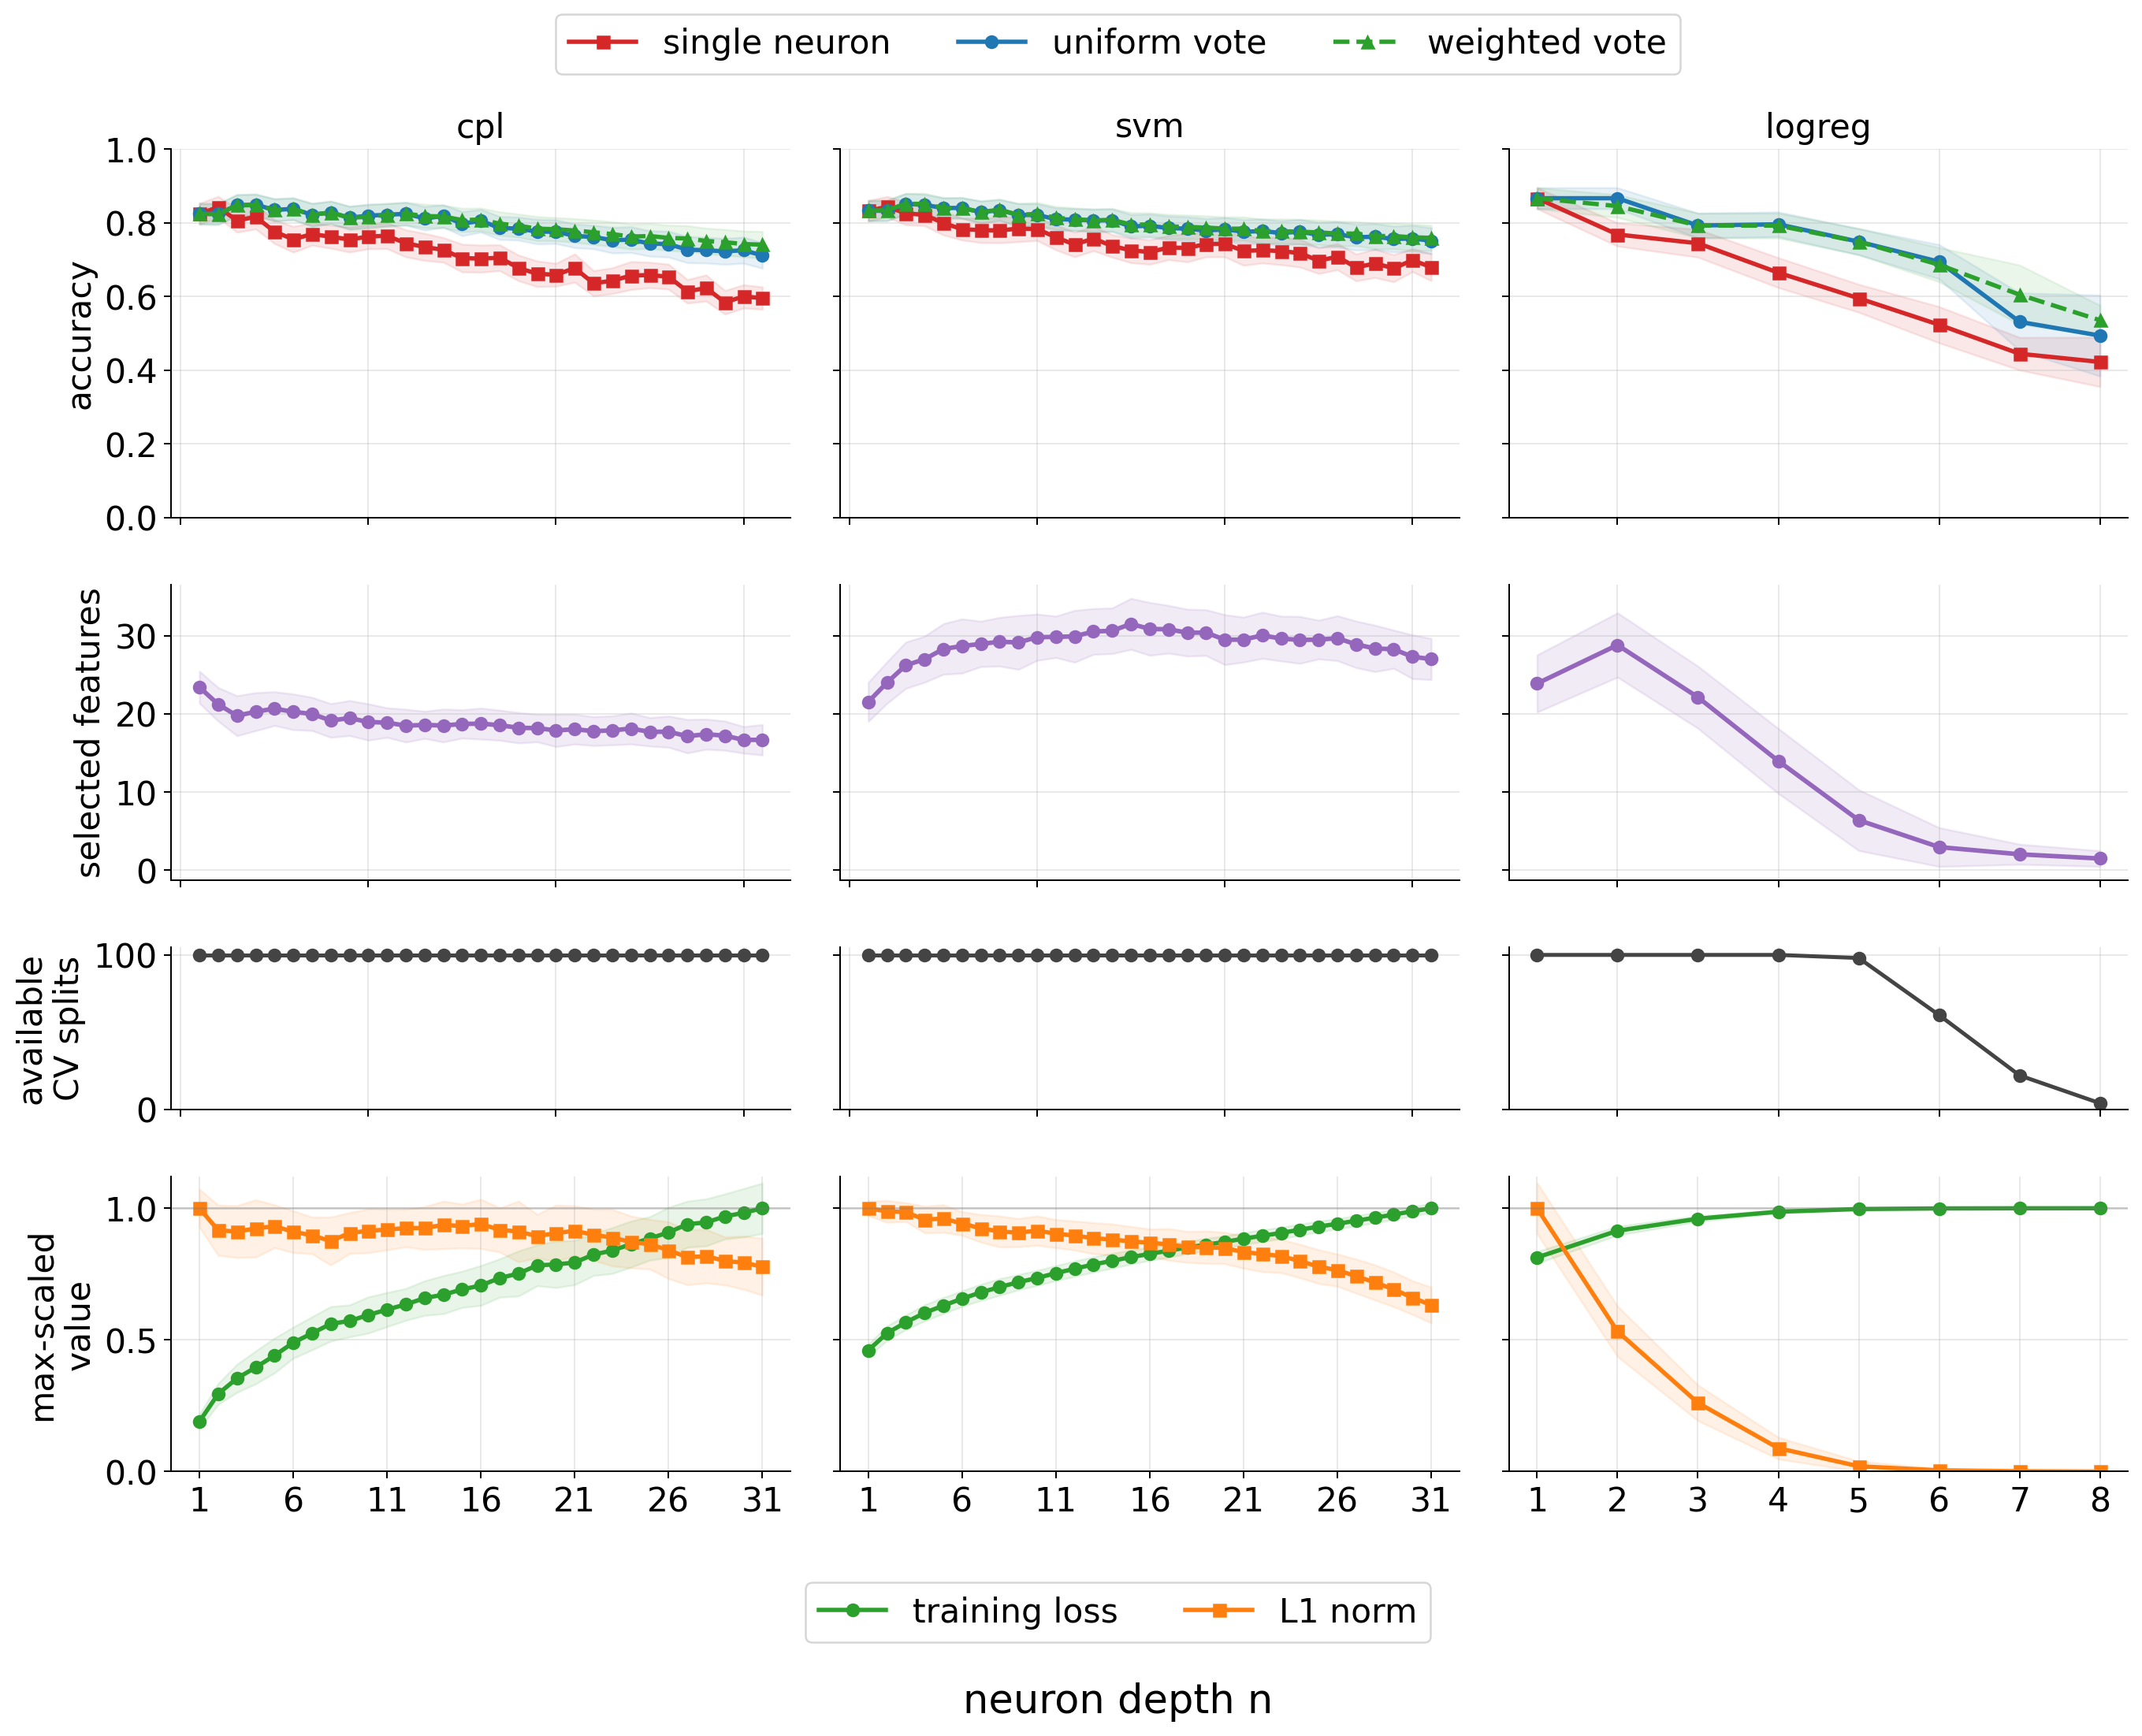
\includegraphics[width=\linewidth]{figures/colon_diagnostics_high.png}
\caption{High-feature diagnostic trajectories on the colon cancer benchmark. Columns show \texttt{cpl},
\texttt{svm}, and \texttt{logreg} with $C_{\mathrm{high}}$. Rows follow the same structure as
Figure~\ref{fig:colon_sparse_accuracy}: predictive accuracy, the average number of features selected by the
$n$-th neuron, the number of CV splits in which that neuron depth was available, and max-scaled optimization
diagnostics for the $n$-th neuron.}
\label{fig:colon_sparse_accuracy_high}
\end{figure}

\begin{figure}[!htbp]
\centering
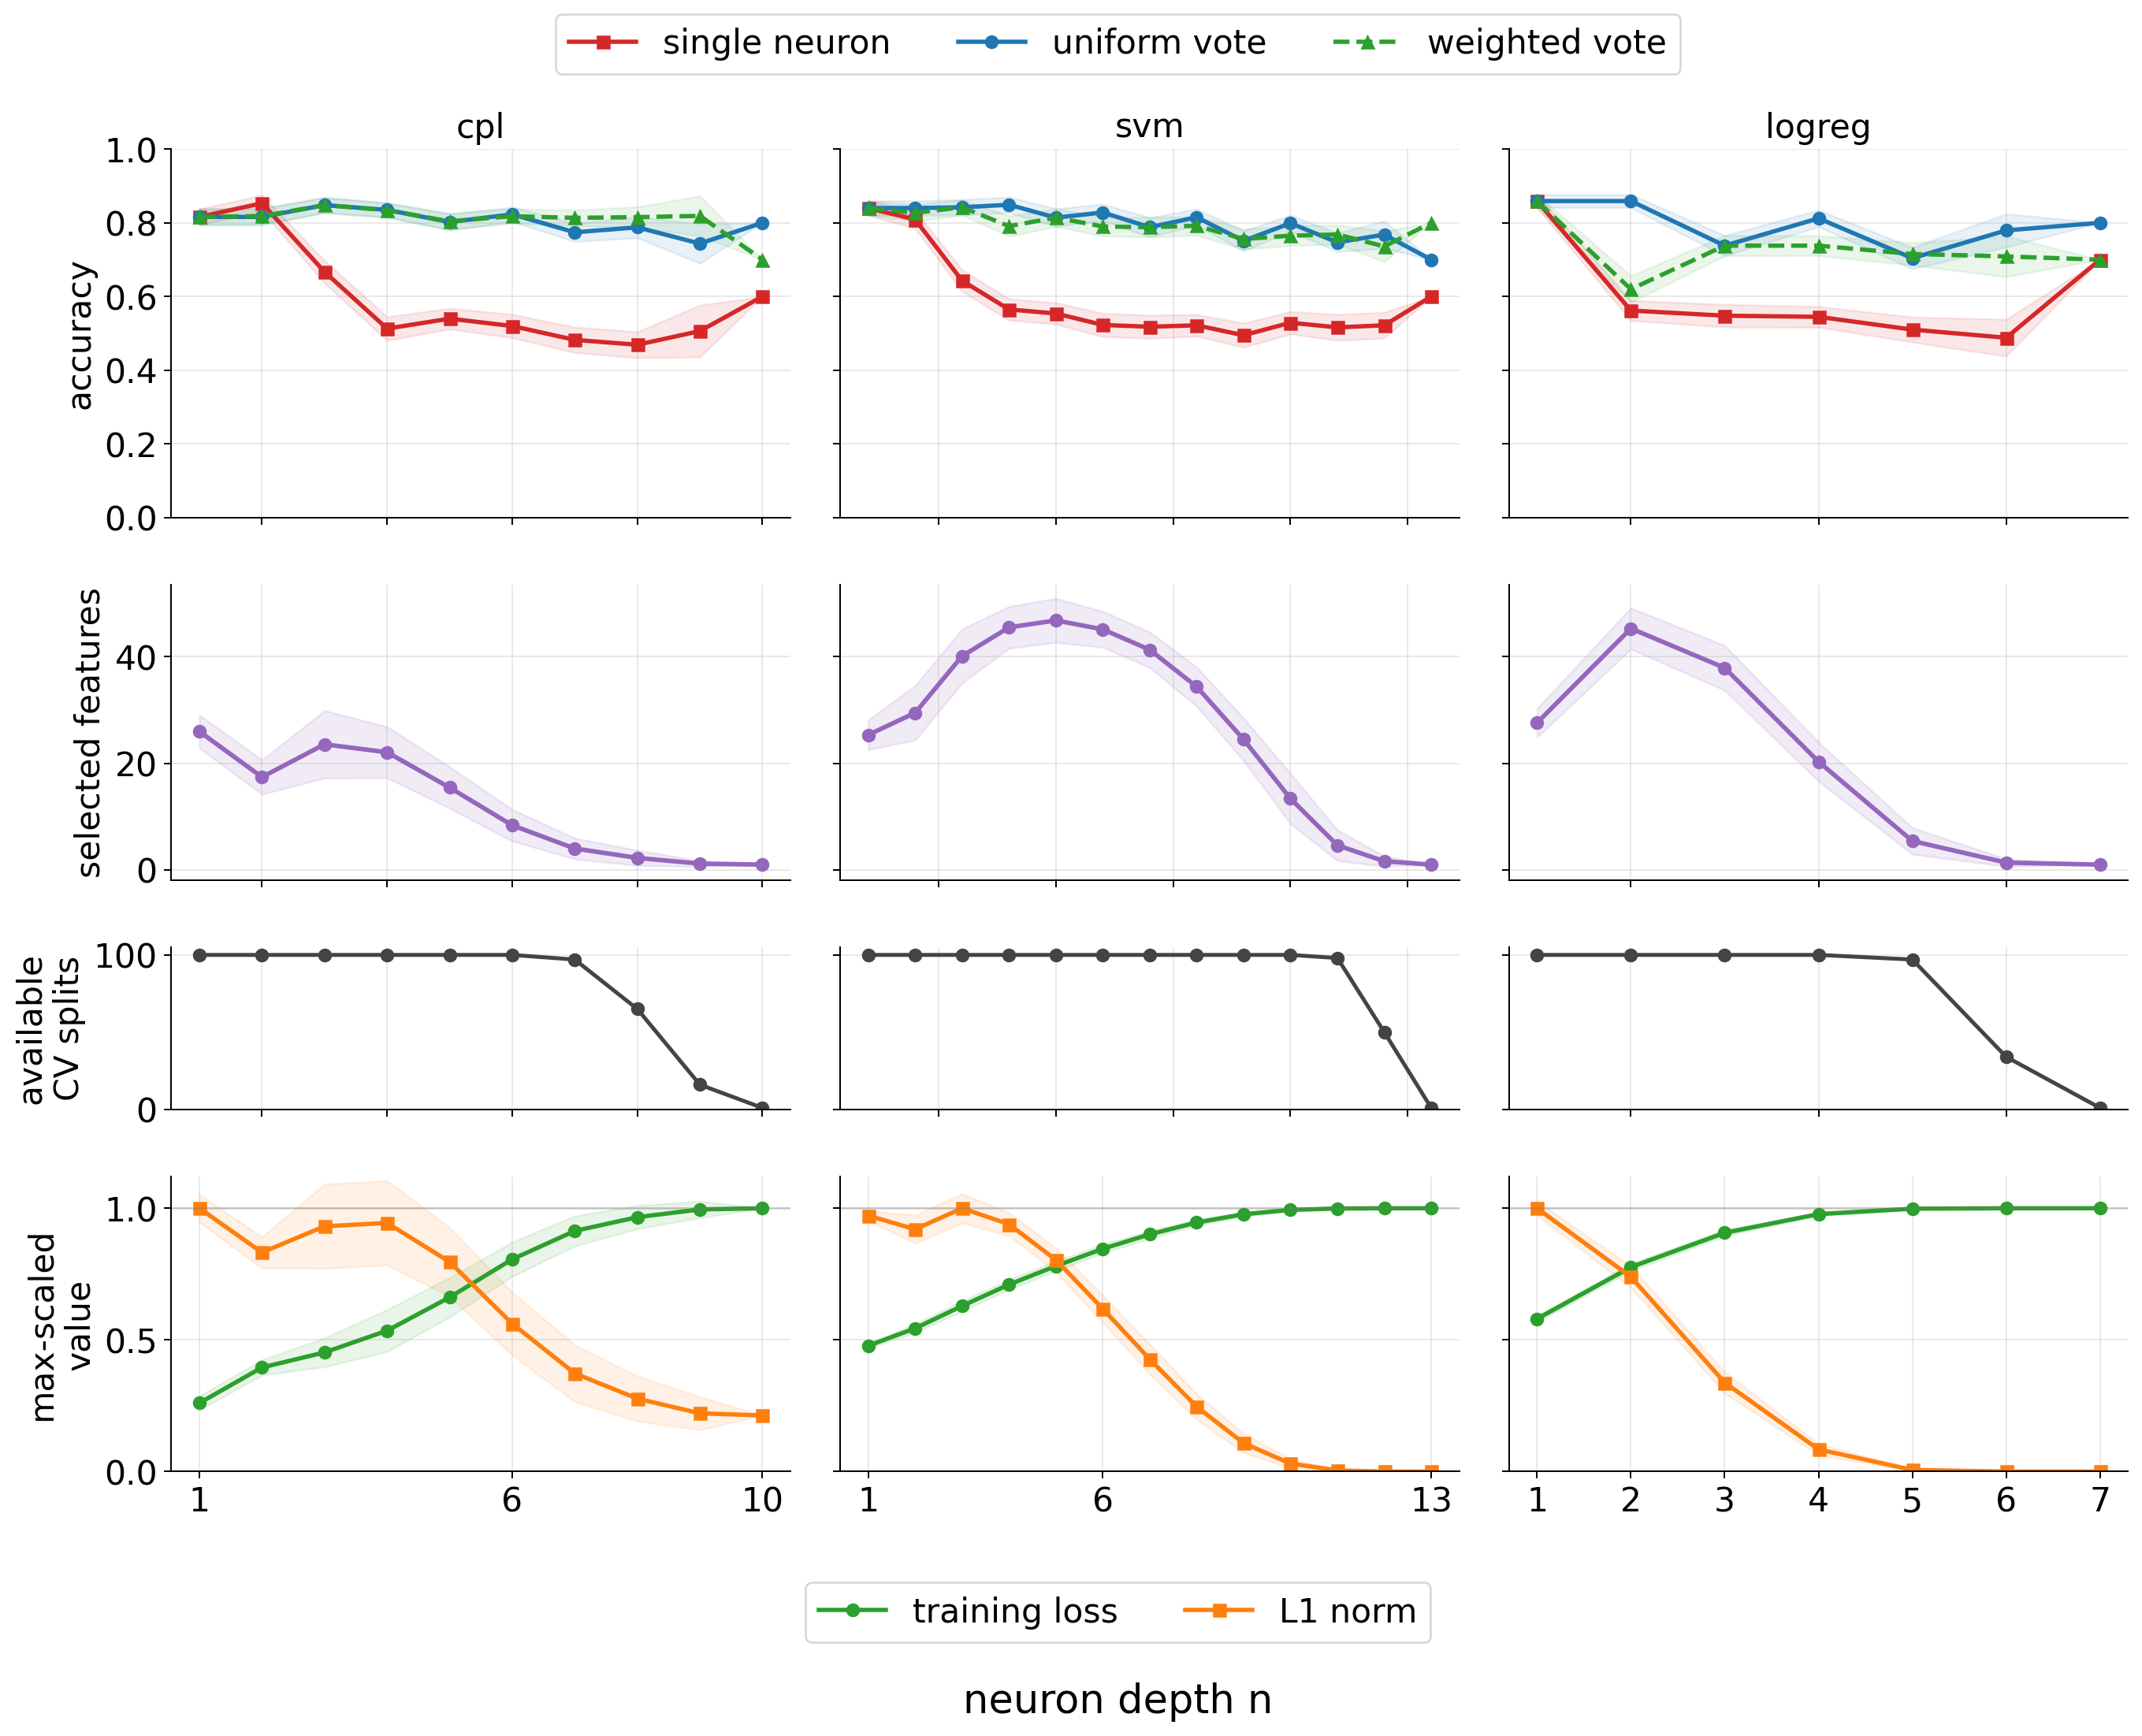
\includegraphics[width=\linewidth]{figures/synthetic_diagnostics_high.png}
\caption{High-feature diagnostic trajectories on the synthetic benchmark. Columns show \texttt{cpl},
\texttt{svm}, and \texttt{logreg} with $C_{\mathrm{high}}$. Rows follow the same structure as
Figure~\ref{fig:synthetic_sparse_accuracy}: predictive accuracy, the average number of features selected by the
$n$-th neuron, the number of CV splits in which that neuron depth was available, and max-scaled optimization
diagnostics for the $n$-th neuron.}
\label{fig:synthetic_sparse_accuracy_high}
\end{figure}

\begin{figure}[!htbp]
\centering
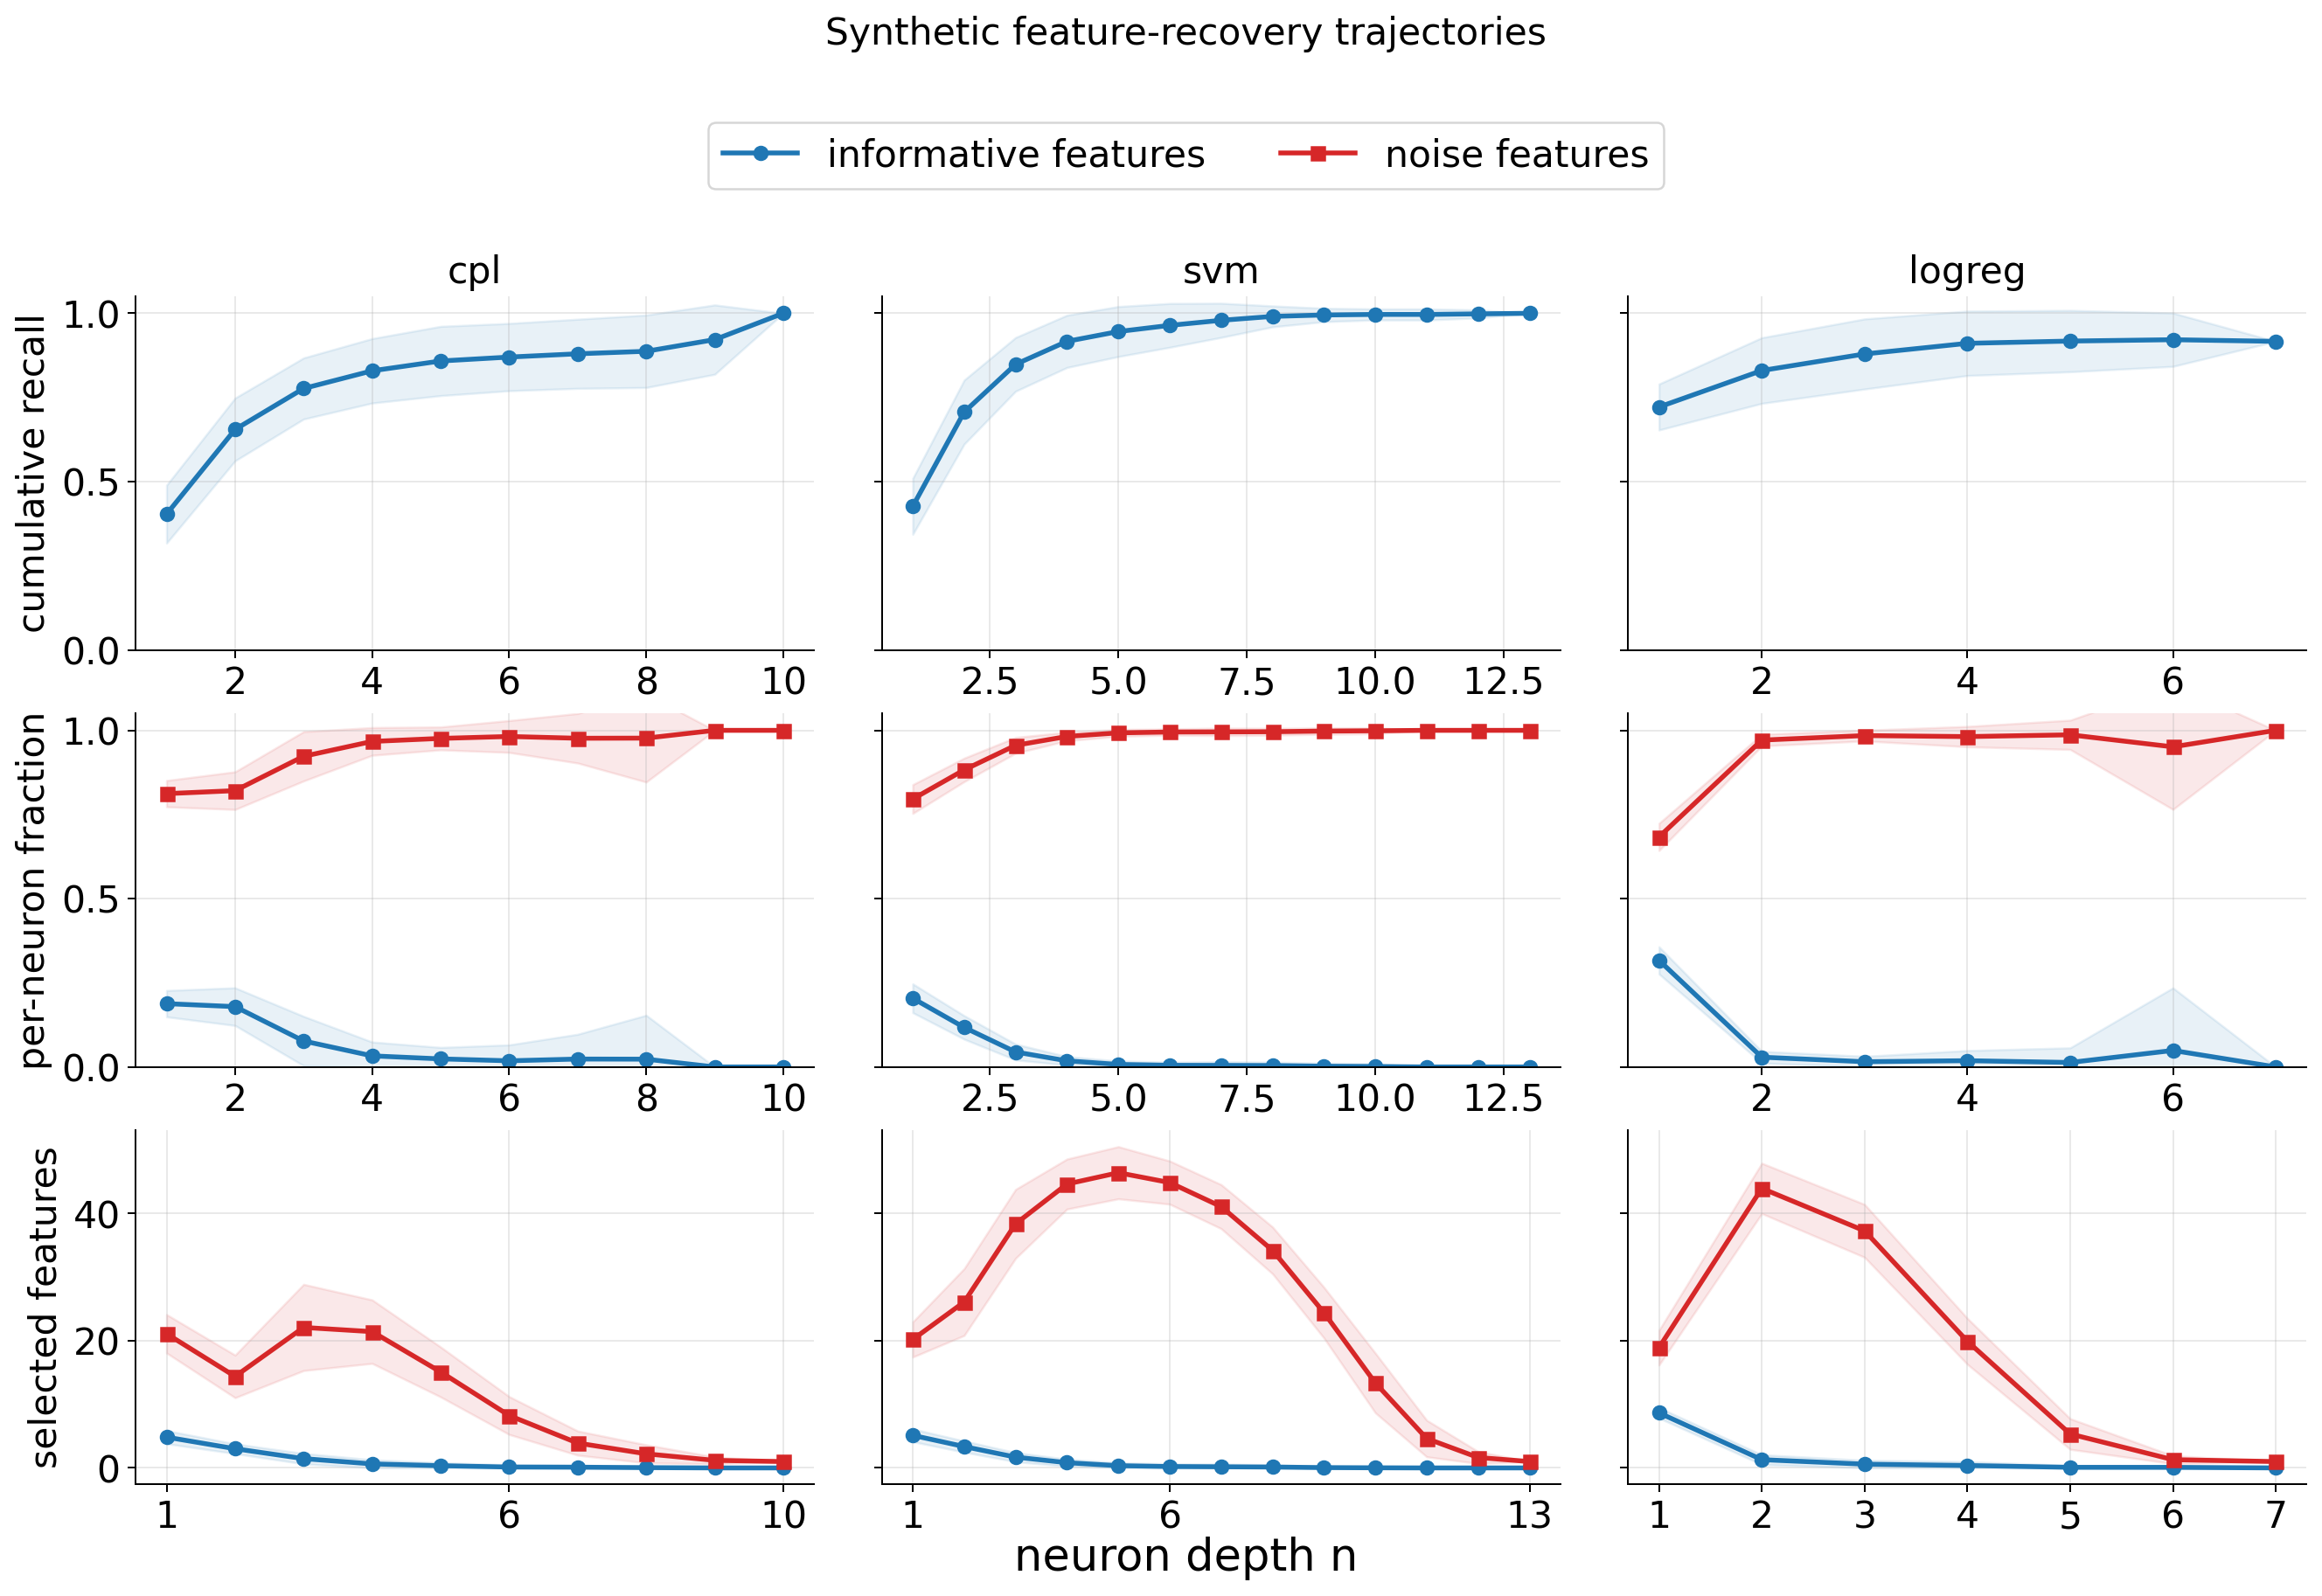
\includegraphics[width=\linewidth]{figures/synthetic_recovery_high.png}
\caption{Feature-recovery trajectories for the high-feature synthetic benchmark. Columns show \texttt{cpl},
\texttt{svm}, and \texttt{logreg} with $C_{\mathrm{high}}$; rows report cumulative informative-feature recall,
per-neuron informative and noise fractions, and the numbers of informative and noise features selected by the
$n$-th neuron. Blue trajectories describe informative features and red trajectories describe noise features.}
\label{fig:synthetic_sparse_recovery_high}
\end{figure}
